\tikzset{every picture/.style={line width=0.75pt}} %set default line width to 0.75pt        

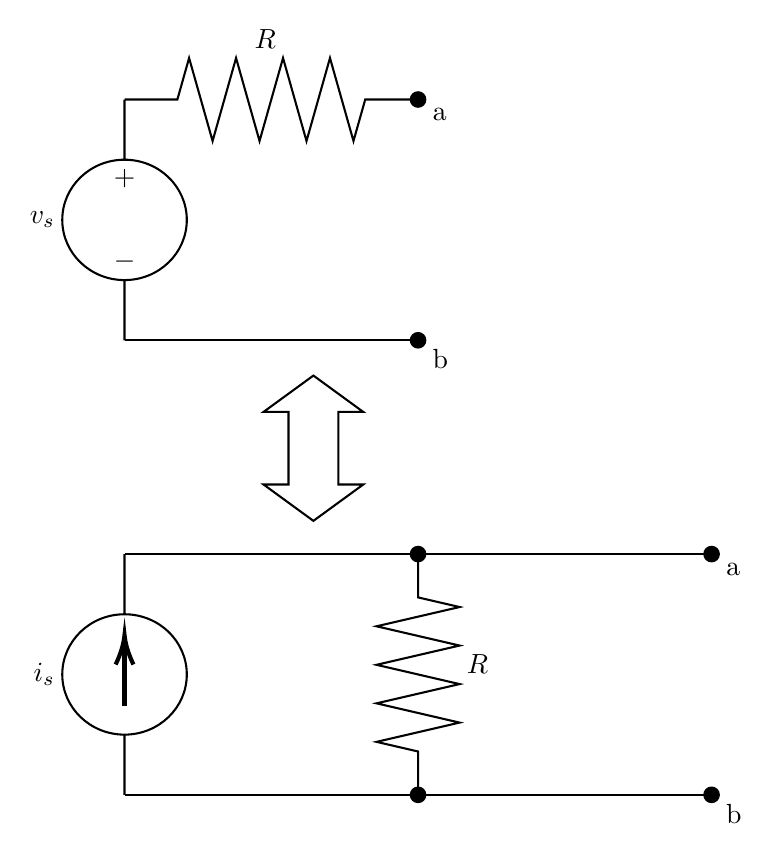
\begin{tikzpicture}[x=0.75pt,y=0.75pt,yscale=-1,xscale=1]
%uncomment if require: \path (0,508); %set diagram left start at 0, and has height of 508

%Shape: Output [id:dp4761018043956171] 
\draw   (119,130) .. controls (135.57,130) and (149,142.98) .. (149,159) .. controls (149,175.02) and (135.57,188) .. (119,188) .. controls (102.43,188) and (89,175.02) .. (89,159) .. controls (89,142.98) and (102.43,130) .. (119,130) -- cycle (119,101) -- (119,130) (119,217) -- (119,188) ;
%Straight Lines [id:da18038673316668685] 
\draw    (260.42,217) -- (119,217) ;
%Shape: Resistor [id:dp49094225036149086] 
\draw   (119,101) -- (144.46,101) -- (150.11,81) -- (161.43,121) -- (172.74,81) -- (184.05,121) -- (195.37,81) -- (206.68,121) -- (217.99,81) -- (229.31,121) -- (234.97,101) -- (260.42,101) ;
%Shape: Circle [id:dp7252316282946523] 
\draw  [fill={rgb, 255:red, 0; green, 0; blue, 0 }  ,fill opacity=1 ] (256.92,101) .. controls (256.92,99.07) and (258.49,97.5) .. (260.42,97.5) .. controls (262.35,97.5) and (263.92,99.07) .. (263.92,101) .. controls (263.92,102.93) and (262.35,104.5) .. (260.42,104.5) .. controls (258.49,104.5) and (256.92,102.93) .. (256.92,101) -- cycle ;
%Shape: Circle [id:dp7082112398028335] 
\draw  [fill={rgb, 255:red, 0; green, 0; blue, 0 }  ,fill opacity=1 ] (256.92,217) .. controls (256.92,215.07) and (258.49,213.5) .. (260.42,213.5) .. controls (262.35,213.5) and (263.92,215.07) .. (263.92,217) .. controls (263.92,218.93) and (262.35,220.5) .. (260.42,220.5) .. controls (258.49,220.5) and (256.92,218.93) .. (256.92,217) -- cycle ;
%Shape: Output [id:dp31169582279695573] 
\draw   (119,349) .. controls (135.57,349) and (149,361.98) .. (149,378) .. controls (149,394.02) and (135.57,407) .. (119,407) .. controls (102.43,407) and (89,394.02) .. (89,378) .. controls (89,361.98) and (102.43,349) .. (119,349) -- cycle (119,320) -- (119,349) (119,436) -- (119,407) ;
%Straight Lines [id:da40535921970588173] 
\draw    (260.42,436) -- (119,436) ;
%Shape: Resistor [id:dp4721611778600978] 
\draw   (260.42,320) -- (260.42,340.88) -- (280.42,345.52) -- (240.42,354.8) -- (280.42,364.08) -- (240.42,373.36) -- (280.42,382.64) -- (240.42,391.92) -- (280.42,401.2) -- (240.42,410.48) -- (260.42,415.12) -- (260.42,436) ;
%Straight Lines [id:da9415238641357673] 
\draw    (401.84,320) -- (260.42,320) ;
%Straight Lines [id:da3487179058682581] 
\draw    (401.84,436) -- (260.42,436) ;
%Shape: Circle [id:dp7676950007550718] 
\draw  [fill={rgb, 255:red, 0; green, 0; blue, 0 }  ,fill opacity=1 ] (256.92,320) .. controls (256.92,318.07) and (258.49,316.5) .. (260.42,316.5) .. controls (262.35,316.5) and (263.92,318.07) .. (263.92,320) .. controls (263.92,321.93) and (262.35,323.5) .. (260.42,323.5) .. controls (258.49,323.5) and (256.92,321.93) .. (256.92,320) -- cycle ;
%Shape: Circle [id:dp7754991479549254] 
\draw  [fill={rgb, 255:red, 0; green, 0; blue, 0 }  ,fill opacity=1 ] (256.92,436) .. controls (256.92,434.07) and (258.49,432.5) .. (260.42,432.5) .. controls (262.35,432.5) and (263.92,434.07) .. (263.92,436) .. controls (263.92,437.93) and (262.35,439.5) .. (260.42,439.5) .. controls (258.49,439.5) and (256.92,437.93) .. (256.92,436) -- cycle ;
%Straight Lines [id:da8126562773083341] 
\draw    (260.42,320) -- (119,320) ;
%Shape: Circle [id:dp749150677492284] 
\draw  [fill={rgb, 255:red, 0; green, 0; blue, 0 }  ,fill opacity=1 ] (398.34,320) .. controls (398.34,318.07) and (399.91,316.5) .. (401.84,316.5) .. controls (403.78,316.5) and (405.34,318.07) .. (405.34,320) .. controls (405.34,321.93) and (403.78,323.5) .. (401.84,323.5) .. controls (399.91,323.5) and (398.34,321.93) .. (398.34,320) -- cycle ;
%Shape: Circle [id:dp8460624756938435] 
\draw  [fill={rgb, 255:red, 0; green, 0; blue, 0 }  ,fill opacity=1 ] (398.34,436) .. controls (398.34,434.07) and (399.91,432.5) .. (401.84,432.5) .. controls (403.78,432.5) and (405.34,434.07) .. (405.34,436) .. controls (405.34,437.93) and (403.78,439.5) .. (401.84,439.5) .. controls (399.91,439.5) and (398.34,437.93) .. (398.34,436) -- cycle ;
%Straight Lines [id:da6858366079722793] 
\draw [line width=1.5]    (119,393) -- (119,362) ;
\draw [shift={(119,359)}, rotate = 90] [color={rgb, 255:red, 0; green, 0; blue, 0 }  ][line width=1.5]    (14.21,-4.28) .. controls (9.04,-1.82) and (4.3,-0.39) .. (0,0) .. controls (4.3,0.39) and (9.04,1.82) .. (14.21,4.28)   ;
%Up Down Arrow [id:dp13938108550459183] 
\draw   (186,251.5) -- (210,234) -- (234,251.5) -- (222,251.5) -- (222,286.5) -- (234,286.5) -- (210,304) -- (186,286.5) -- (198,286.5) -- (198,251.5) -- cycle ;

% Text Node
\draw (87,159) node [anchor=east] [inner sep=0.75pt]   [align=left] {$\displaystyle v_{s}$};
% Text Node
\draw (193.37,78) node [anchor=south east] [inner sep=0.75pt]   [align=left] {$\displaystyle R$};
% Text Node
\draw (119,133) node [anchor=north] [inner sep=0.75pt]   [align=left] {\begin{minipage}[lt]{8.68pt}\setlength\topsep{0pt}
\begin{center}
+
\end{center}

\end{minipage}};
% Text Node
\draw (119,185) node [anchor=south] [inner sep=0.75pt]   [align=left] {$\displaystyle -$};
% Text Node
\draw (87,378) node [anchor=east] [inner sep=0.75pt]   [align=left] {$\displaystyle i_{s}$};
% Text Node
\draw (282.42,367.08) node [anchor=north west][inner sep=0.75pt]   [align=left] {$\displaystyle R$};
% Text Node
\draw (265.92,104) node [anchor=north west][inner sep=0.75pt]   [align=left] {a};
% Text Node
\draw (407.34,323) node [anchor=north west][inner sep=0.75pt]   [align=left] {a};
% Text Node
\draw (265.92,220) node [anchor=north west][inner sep=0.75pt]   [align=left] {b};
% Text Node
\draw (407.34,439) node [anchor=north west][inner sep=0.75pt]   [align=left] {b};


\end{tikzpicture}
